\documentclass[12pt]{article}
\usepackage[margin=1in]{geometry}
\usepackage{natbib}
\usepackage{graphicx}
\usepackage{caption}
\usepackage{subcaption}
\usepackage{multirow}
\usepackage{longtable}
\usepackage{color}
\usepackage{hyperref}
\bibliographystyle{apalike}
\newcommand{\beginsupplement}{%
        \setcounter{table}{0}
        \renewcommand{\thetable}{S\arabic{table}}%
        \setcounter{figure}{0}
        \renewcommand{\thefigure}{S\arabic{figure}}%
     }
\newcommand{\citex}{\textcolor{red}{\bf CITE}}
\newcommand{\X}{\textcolor{red}{\bf X}}

\begin{document}

\title{Evolutionary genomics of peach \\and almond domestication}

\author{\small\sfbf{Dianne Velasco$^{\S}$, Mallikarjuna Aradhya$^{\dag}$, Jeffrey Ross-Ibarra$^{\S\ddag}$}\thanks{Corresponding author: Department of Plant Sciences, University of California, Davis, California 95616, USA. E-mail: \mbox{rossibarra@ucdavis.edu}} \\[0.3cm]
     \small\sf $^{\S}$Department of Plant Sciences, University of California, Davis, California 95616, USA,\\
     \small\sf $^{\dag}$USDA-ARS National Clonal Germplasm Repository, Davis, California 95616, USA,\\
     \small\sf $^{\ddag}$Center for Population Biology and Genome Center, University of California, Davis, California 95616, USA}

\date{\today}
%\maketitle
\section*{Introduction}
%BACKGROUND ON SPECIES
%
\emph{Prunus} is the largest genus in the family Rosaceae \citex with approximately four hundred species, including multiple domesticated crops, such as almond, apricot, cherry, cherry, peach, and plum.
%
Peach [\emph{P. persica} (Mill.) D. A. Webb] and almond [\emph{P. dulcis} (L.) Batsch] are sibling species found within the subgenus \emph{Amygdalus}.
%
Peach and almond are similar in many ways, including early fruit development, perenniality, precocity, genome organization \citep{arus2012peach}, and genome size \citep{baird1994estimating}. 
%probably dont need so many cites on genome size.
%
The most striking between the species are mature fruit morphology and mating systems: peaches are harvested for their indehiscent fleshy mesocarp while almonds are harvested for the stony endocarp encased seeds obtained from within the leathery dehiscent mesocarp and exocarp. 
%
But almond and peach also differ for other traits, such as life span, chilling requirement, and adventitious root generation.
%
The natural life span of almonds may exceed 100 years \citex,
%http://www.european-trees.com/almond.html ; literature sources not easy to locate, will continue to look
%commercial life span of 20-25 years, but this may be mostly due to peach or peach-derived rootstocks and peak bearing period
flowering initiation requires only 400-600 hours chilling \citep{alonso2005determination}, 
% versus peach <650-1050 /citep{dozier1990hydrogen}
and less adventitious root generation \citex when compared to the peach life span of 25-30 years\citex, 
%is this primarily commercial production life span?
%how are they "in the wild"?
600-1000 hours of required chilling \citex, 
%have maybe seen a bit lower
and good adventitious rooting ability \citex. 
%
Additionally, while \emph{Prunus} species generally exhibit gametophytic self-incompatibility, peach is fully self-compatible.

%each sentence on different line is helpful, but no need to put % between each sentence
% I found that I could find lines faster/easier this way

Domestication of almond and peach occurred approximately 5000 BP in the Fertile Crescent and China \citep{zohary2012domestication}, respectively, followed by global dissemination beginning before 2300 BP \citep{hedrick1917peaches, edwards1975almond, gradziel2011origin, zheng2014archaeological}. 
%peach recorded dissemination to Persia by 332 BC, Rome by 79 AD, France from 530 to 784 AD, and the Americas by the 16th century
%Nice peach generation time description: "a peach falling to the ground brings a peach tree that shall bear in three years, or sometimes sooner" Hedrick p45 quoting John Lawson (1700)
%Lawson also described the peach tendency of overabundance: "They generally bear so full that they break great part of their limbs down"
%Lawson's statements also suggest the degree of inbreeding in Indian/American peaches: "we generally raise this fruit from the stone, which never fails to bring the same fruit" Hedrick p46
%grafting in the Americas was becoming more common practice by the end of the 18th century (Hedrick p57)
%
%Wikipedia regarding Turkestan: "includes [parts to all of] present-day Turkmenistan, Kazakhstan, Uzbekistan Kyrgyzstan, and Xinjiang ("Chinese Turkestan")" and "acquired its "Turkic" character from the 4th to 6th centuries AD with the incipient Turkic expansion" although the Turkic peoples are purported to originate in the Altai Mountains (north of the east end of the Taklamakan Desert and west of the Gobi Desert) currently in China (?; Kashgar?) and origin of Uygur peoples
%Uygurs have a strong affiliation with almond, but many of their traditions are similar to those of Western Asia and Mediterranean Europe, so West to East or East to West?
%The Taklamakan Desert, or rather oases throughout, funneled the various silk routes through that desert and surrounding mountain ranges
%
The few obvious traits associated with almond domestication are reduced toxicity, thinner endocarp, and increased seed size, while domestication in peach is characterized by diverse fruit morphology (size, color, texture, shape, etc.) and self-compatibility.
%
However, traits not typically associated with domestication but common to both, such as precocity, or solely with peach, such as relative ease of adventitious rooting, may have also been targeted or incidentally selected during domestication. 
%
Unfortunately, efforts to identify wild progenitors of almond and peach \citep{verde2013high, aradhya2004molecular, zeinalabedini2010origin, mowrey1990isozyme, browicz1996genus, ladizinsky1999origin, bassi20081} by examining species relationships within the subgenus \emph{Amygdalus} have had mixed results. 
%
Given the uncertainty in identifying wild progenitors of almond and peach, domestication studies using crossing experiments are not suitable and are generally impractical in perennial crops.
%crossing experiment citation, perhaps one of Doebley's papers or others using domesticated x wild cross to identify domestication locus/loci (maize, tomato, etc.)
%
With the recent cost reductions in high throughput sequencing, using genomic resequencing is a practical approach to gain insights into domestication of perennial crops and its genome-wide nature also enables distinguishing between mating system and domestication effects. 
%
Both domestication and mating system have been shown to shape genome diversity in annual species \citep{glemin2006impact, doebley2006molecular, slotte2013capsella}, but the impacts of these forces on tree species remains poorly understood \citep{mckey2010evolutionary, miller2011forest}.


%DOMESTICATION VERSUS SI/SC IN GENOME
In closely related species pairs with alternate mating systems, such as \emph{Arabidopsis thaliana} and \emph{A. lyrata} and \emph{Capsella rubella} and \emph{C. grandiflora} \citep{slotte2013capsella}, mating system is shown to significantly affect genome evolution, as evidenced by nucleotide diversity, linkage disequilibrium (LD), heterozygosity, genome size, repeat content, and genetic load.
%
We thus expect that that self-compatible peach has lower genome-wide diversity than self-incompatible almond.
%
However, domestication also reduces genomic diversity genome-wide due to reduced effective population size \citex and in localized regions important to domestication \citep{glemin2006impact, doebley2006molecular}. 
%demographic effects associated
%Though both peach and almond have undergone domestication, only localized reductions in genomic diversity will be due to domestication while large, genome-wide differences are due to alternate mating systems \citep{glemin2006impact, charlesworth2001breeding}. 
%
%Domestication in plants is associated with changes in many traits, such as increased size and morphological diversity of the harvested organ (seed, fruit, leaves, etc.), reduced seed dispersal, adaptation to disturbed environments, reduced toxicity, selfing, photoperiod insensitivity, etc. \citep{doebley2006molecular}, but a relative few of these changes are striking in almond or peach. 
%
%seed size in almond, fruit size & color in peach
%range of bloom/maturity dates for peach
%sweet kernels in almond
%what about other tree crops? (Review Miller & Gross paper)
%
%STUDY PURPOSE AND SUMMARY
%
Like all species within the subgenus \emph{Amygdalus}, peach and almond are both diploid, and genetic mapping from an almond x peach $F_{2}$ population suggests they have a similar genomic structure \citep{dirlewanger2004comparative}. 
%
At an estimated 230 Megabases (Mb) spanning eight chromosomes, the recently sequenced peach genome \citep{verde2013high} is less than double the genome size of model plant \emph{Arabidopsis thaliana}. 
%
At 300 Mb the cytologically estimated almond genome size is similar to pre-sequencing estimates of peach \citep{arumuganathan1991nuclear}. 
% efficient species
%
%Peach already serves as a model system for \emph{Prunus} and other tree crops due to its small genome (230 Mb), short generation time (2-3 years), and self-compatibility \citep{arus2012peach}.
%
%Small genome sizes, chromosome numbers, and relatively short juvenility, peach and almond support their use as a model to investigate the effects of domestication and mating system in trees.
%
Recent analysis of resequenced peach genomes indicates low genetic diversity and higher LD across the genome compared to wild peach species \citep{verde2013high}, but the few resequenced almond genomes have not been similarly assessed. 
%
%This is not unexpected considering the primary peach genetic map is based on an almond x peach $F_2$ population due to poor resolution in peach $F_2$ genetic maps \citep{arus2012peach, joobeur1998construction, aranzana2003set, dirlewanger2004comparative, dominguez2003plant}.
%
%However, due to self-incompatibility almond is expected to have higher levels of heterozygosity and lower LD compared to peach.
%
Understanding the impact of mating system on almond and peach evolutionary genomics expands the basic understanding of genome evolution in a perennial species pair with alternate mating systems. 
%is this a first for perennial species? <-- DUNNO, THAT WOULD BE COOL!
%
Identification of candidate domestication loci will provide an opportunity to determine which loci in almond and peach were under selection, if any are in common, and to identify similarities or differences when compared to annual crops. 
%Knowledge gained from these analyses provides valuable information regarding domestication loci and haplotypes, an important resource for tree breeding programs.
%Understanding the contributions of domestication and mating systems to genome evolution in almond and peach expands the understanding of these processes beyond annual species. 
Here we present an evolutionary genomic analysis of the effects of domestication and mating system on genomic diversity in peach and almond, providing a model for  future analysis of evolution and domestication in other tree species.
%
\\
\section*{Materials and Methods}
%
\subsection*{Samples}
We resequenced nine \emph{P. dulcis}, one \emph{P. persica}, one closely related species, \emph{P. fenzliana}, and one plum outgroup species, \emph{P. cerasifera}, for analysis.
%
All were paired end 100 bp sequenced with Illumina HiSeq 2000. 
%
Of these samples, eight \emph{P. dulcis} were sequenced at the Vincent J. Coates Genomics Sequencing Laboratory at UC Berkeley from libraries prepared in our laboratory. 
%Anne's library prep <- need reference or details
%sheared X cycles for X seconds per cycle with a Bioruptor; end repair, adapter ligation, amplification; plus clean up and size selection along the way
% QC with a BioAnalyzer and qPCR for pooling 
%
DNA of the remaining four samples was submitted to BGI (Shenzen, China) 
% Shenzen correct??
for library preparation and sequencing at their facility.
% In the we sequenced paragraph you need to provide PE 100, where they were sequenced, what average depth, and a citation for library prep (or if we paid someone to prep libraries)
%

Additionally, we utilized five resequenced \emph{P. dulcis} genomes from public sources, four from \citealt{koepke2013comparative} 
%(?)
the NCBI Sequence Read Archive (SRA) and one from the RosBREED group FTP site.
% include URL or something?
%
We downloaded thirty-one resequenced \emph{P. persica}, thirteen from the NCBI SRA (ten from \citealt{verde2013high} and three from \citealt{ahmad2011whole}) and eighteen from RosBREED.
%
One wild peach species, \emph{P. ferganensis}, was publicly available from NCBI SRA \citep{verde2013high}.\\
%
%
\subsection*{Analysis}
\emph{Sequencing, Quality Control, and Mapping}

All publicly available resequenced samples were paired end but varied in length from 80 to 100 bp in read length. 
% recheck this range
%
Regardless of source all FASTQ files were trimmed of remnant adapter sequences using Scythe and then further trimmed using base quality with Sickle. 
%
% Buffalo V: Scythe. [https://github.com/vsbuffalo/scythe]
% figure out citation for Scythe; include version
%
% Najoshi :Sickle [https://github.com/najoshi/sickle]
% same as for Scythe
%
Trimmed reads were then aligned to the peach v 1.0 reference using BWA-MEM using a minimum seed length of 10 and internal seed length of 28.5.
% using -k 10 -r 2.85 parameters
% -k INT		minimum seed length [19]
% -r FLOAT	look for internal seeds inside a seed longer than {-k} * FLOAT [1.5]
% internal seed length remains the same as default parameters
% picked this up from P. Morrell
%
 \citep{li2013aligning}. 
% bwa mem -k 10 -r 2.85
% provide explanation of parameters
%
\\
\emph{SNP calling}

%If going this route
%
%SNP calling using SAMtools pileup and BCFtools \citep{li2009sequence} \\
% may change to ANGSD
%
%PopBAM analysis: SAMtools was used to merge bams and add new header \citep{li2009sequence} with appropriate sample and population information for use in PopBAM \citep{garrigan2013popbam}. 
%SNPs called in PopBAM were output in the SweepFinder \citep{nielsen2005genomic} format and then analyzed.\\
% if not switching to ANGSD
%
Genotype likelihoods were first called using ANGSD \citep{korneliussen2014angsd}.
%
Inbreeding coefficients were estimated using \emph{ngsF} from the \emph{ngsTools} \citep{fumagalli2014ngstools} suite.
%
SNPs and genotype likelihoods were called utilizing the estimated inbreeding coefficients.
\\
%
\\
\emph{Diversity Evaluation}

Using ANGSD genotype likelihoods and posterior probabilities we calculated several population genetics statistics, such as Watterson's theta ($\theta_{W}$) \citex and pairwise nucleotide diversity ($\theta_{\pi}$) \citex, and neutrality deviation tests, such as Tajima's D \citex, Fay's H (Fay and Wu's H, right?) \citex, and Zeng's E \citex.
\\
%
\\
\emph{Population Comparisons}

We treated peach and almond samples as belonging to two populations to understand population structure, assign population proportions, and determine population differentiation.
% covar with ngsPopGen, admixture with NGSadmix, Fst with ANGSD
% perhaps put the software with the specific analysis instead of intro sentence
%
First we performed a principal component analysis (PCA) with \emph{ngsPopGen} \citex to determine any underlying population structure.
%might show clear distinction between groups, possibly some overlap
%
Next we used \emph{NGSadmix} \citep{skotte2013estimating} to assign almond and peach population proportions (\emph{K} = 2) to individuals. 
%
Proportion assignment accuracy was evaluated utilizing the sequence of a previously identified F1 peach-almond hybrid and a peach variety with known almond ancestry three generations prior in its pedigree.
% still need to perform witht the peach containing introgressed almond
%
Finally, we examined population differentiation using F$_{ST}$ as determined by ANGSD.
% 6/17 worked, uses a lot of memory - probably want to change the windows and step parameters, which were 50000 and 10000, to something like 1000 and 200
%
\\
%
\\
\emph{Identification of Selected Loci}

Genome-wide population genetics statistics (thetaPi, thetaW, Fay \& Wu's H, Zeng's E) were calculated in 1000 bp windows with 50 bp steps using the \emph{ngsTools} \citep{fumagalli2014ngstools} suite.
%
Regions of possible selection interest determined using Zeng's E statistic \citep{zeng2006statistical} from windows with more than 100 sites per window.
%
Intersections of windows with the Prunus persica v 1.0 genes GFF3 file using bedtools \citep{quinlan2010bedtools} identified genic and non-genic windows.
%
Separation and merging of genic windows by gene ID allowed the calculation of mean genic Zeng's E and identification of genes of interest in the 1\% and 5\% quantiles.
\\
%
\\
\emph{Gene Ontology Analysis}

Gene ontology (GO) term analysis using singular enrichment analysis analysis tool and \emph{P. persica} protein IDs at the AgriGO website (http://bioinfo.cau.edu.cn/agriGO/) identified.
%
Genes with low Zeng's E scores were divided into three categories, shared in both almond and peach, and genes unique to either almond or peach. 
%
Each of the three identified gene categories were analyzed independently. 
%
Genes with significant scores were identified by both p-value and FDR.
\\
%
\\
\begin{center}
\begin{longtable}{lllll}
\caption[P. dulcis, P. persica and related species used in analysis.]{\emph{P. dulcis}, \emph{P. persica} and related species used in analysis.} \label{my-label} \\
\hline \hline \multicolumn{1}{l}{\textbf{Species}} &
\multicolumn{1}{l}{\textbf{Number}} &
\multicolumn{1}{l}{\textbf{Source}} &
\multicolumn{1}{l}{\textbf{Reference}}\\ \hline 
\endfirsthead

\multicolumn{4}{r}{{\bfseries \tablename\ \thetable{} -- continued from previous page}} \\
\hline \multicolumn{1}{l}{\textbf{Species}} &
\multicolumn{1}{l}{\textbf{Number}} &
\multicolumn{1}{l}{\textbf{Source}} &
\multicolumn{1}{}{\textbf{Reference}} \\ \hline 
\endhead

\hline \multicolumn{4}{r}{{Continued on next page}} \\ \hline
\endfoot

\hline \hline
\endlastfoot

                 %\multicolumn{4}{l}
                  \emph{P. dulcis} &4 &NCBI SRA &\citealt{koepke2013comparative}\\
                  \emph{P. dulcis} &1 &RosBREED &URL\\
                  \emph{P. dulcis} &8 &UC Berkeley &this study \\
                  \emph{P. dulcis} &1 &BGI &this study\\
                 %\multicolumn{4}{l}
                  \emph{P. persica} &10 &NCBI SRA &\citealt{verde2013high} \\ % format italics
                  \emph{P. persica} &3 &NCBI SRA &\citealt{ahmad2011whole} \\ % format italics
                  \emph{P. persica} &18 &RosBREED &URL \\ % format italics
                  \emph{P. persica} &1 &BGI &this study \\ % format italics
                 %Almond Board resequencing (performed at BGI)
                 \emph{P. fenzliana} &1 &BGI &this study\\
                 %UCD,ABC
                 \emph{P. ferganensis} &1 &NCBI SRA &\citealt{verde2013high}\\
                 \emph{P. cerasifera} &1 &BGI &this study\\ \hline
                 %outgroup
                 %NCBI SRA
               %note that the SRR IDs are from NCBI SRA
               %GDR/RosBREED (ftp://ftp.bioinfo.wsu.edu/species/Prunus_persica/RosBREED_Illumina/)

\end{longtable}
\end{center}


%add indicator whether sample was plant material or public sequence (reference does give some indication or possibly just put indication that when "this study" is the reference that it indicates that plant material was used)

\section*{Results}
\emph{Quality Control and Mapping}\\

Depth and alignment from SAMtools using depth and flagstat subprograms \citep{li2009sequence} determined a mean mapped sequence depth of 10.710, which ranged from 1.138 to 37.358 (supp. Figure \ref{fig:depth}).
%should separate out for our sequenced stuff and all else
% with outgroup and "progenitor" sequences
% mean mapped sequence depth of 11.719, which ranged from 1.138 to 37.358
% mean mapped persica was 8.917, ranged from 1.138 to 35.358
% mean mapped dulcis was 14.808, ranged from 2.196 to 34.593
%
% below are for all sequenced samples, which includes those not in the study set
% BQ20: mean 27.212, range 7.169 to 48.039 \\
% BQ20MQ20: mean 22.29, range 4.948 to 41.552\\
% BQ20MQ30: mean 21.759, range 4.715 to 41.105\\
% Should this be in Results section instead?
%
% several custom scripts (deposit to github repo, add URL) were used for initial processing of data or to extract data for downstream use\\
Depth etc.\\
%
\\
\emph{SNP calling}\\
%hmmm what to say
\\
%
\\
\emph{Peach and Almond Diversity and Population Comparisons}

Nucleotide diversity ($\theta_{\pi}$) was higher in almond than peach, with genome-wide means of 0.0186 and 0.0035, respectively. 
%
Mean per chromosome $\theta_{\pi}$ ranged from 0.0163 to 0.0219 in dulcis, and from 0.0028 to 0.0047 in persica.
Additional statistics: Watterson's theta ($\theta_{W}$)
Neutrality tests: Tajima's D, Fay's H (=Fay and Wu's H, right?), and Zeng's E
For the admixture results individuals were clearly assigned to either peach or almond populations. 
%
The previously identified peach-almond F1 hybrid was assigned as 0.4758 dulcis and 0.5242 persica, while the peach with introgressed almond ancestry was assigned as X dulcis and Y persica.
%TBD
%

F$_{ST}$: unweighted 0.029449; weighted 0.668699
\\
%
\\
\emph{Selected Loci and Gene Ontology}\\
Of the 27256 genes on chromosomes one through eight, dulcis and persica had 265 and 268 genes, respectively, in the 1\% quantile. 
%total genes on all chromosomes \& scaffolds: 27864\\
%
Twenty-nine of those genes are shared between dulcis and persica.
%
In the 5\% quantile dulcis and persica had 1325 and 1340 genes of interest, respectively, with 286 shared.
\\


\section*{Discussion}
As expected, given its self-compatibility, the genome-wide mean nucleotide diversity in peach is lower than almond.
%
\\
Peach and almond also share more genes of interest in common than expected.
% for sibling species?
%

\pagebreak
%\bibliographystyle{apalike} %can use here and not in header
\bibliography{references.bib}
%
%FIGURE EXAMPLE
%demographic effects (Figure \ref{fig:peach}) can impact deleterious allele distro
%
%SUBSCRIPT EXAMPLE
%$V_a$ influenced by demography\\
%
\pagebreak
\begin{figure}[b]
\centering
   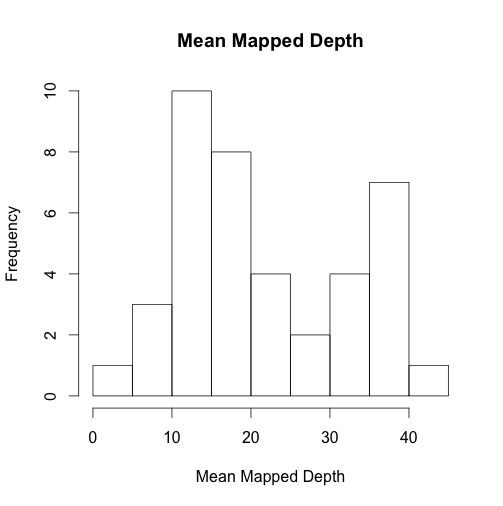
\includegraphics[width=0.8\textwidth]{depthBQ20MQ30.png}
  \caption{Mean mapped depth of sequenced used in analysis}
  \label{fig:depth}
\end{figure}

\begin{figure}[b]
\centering
   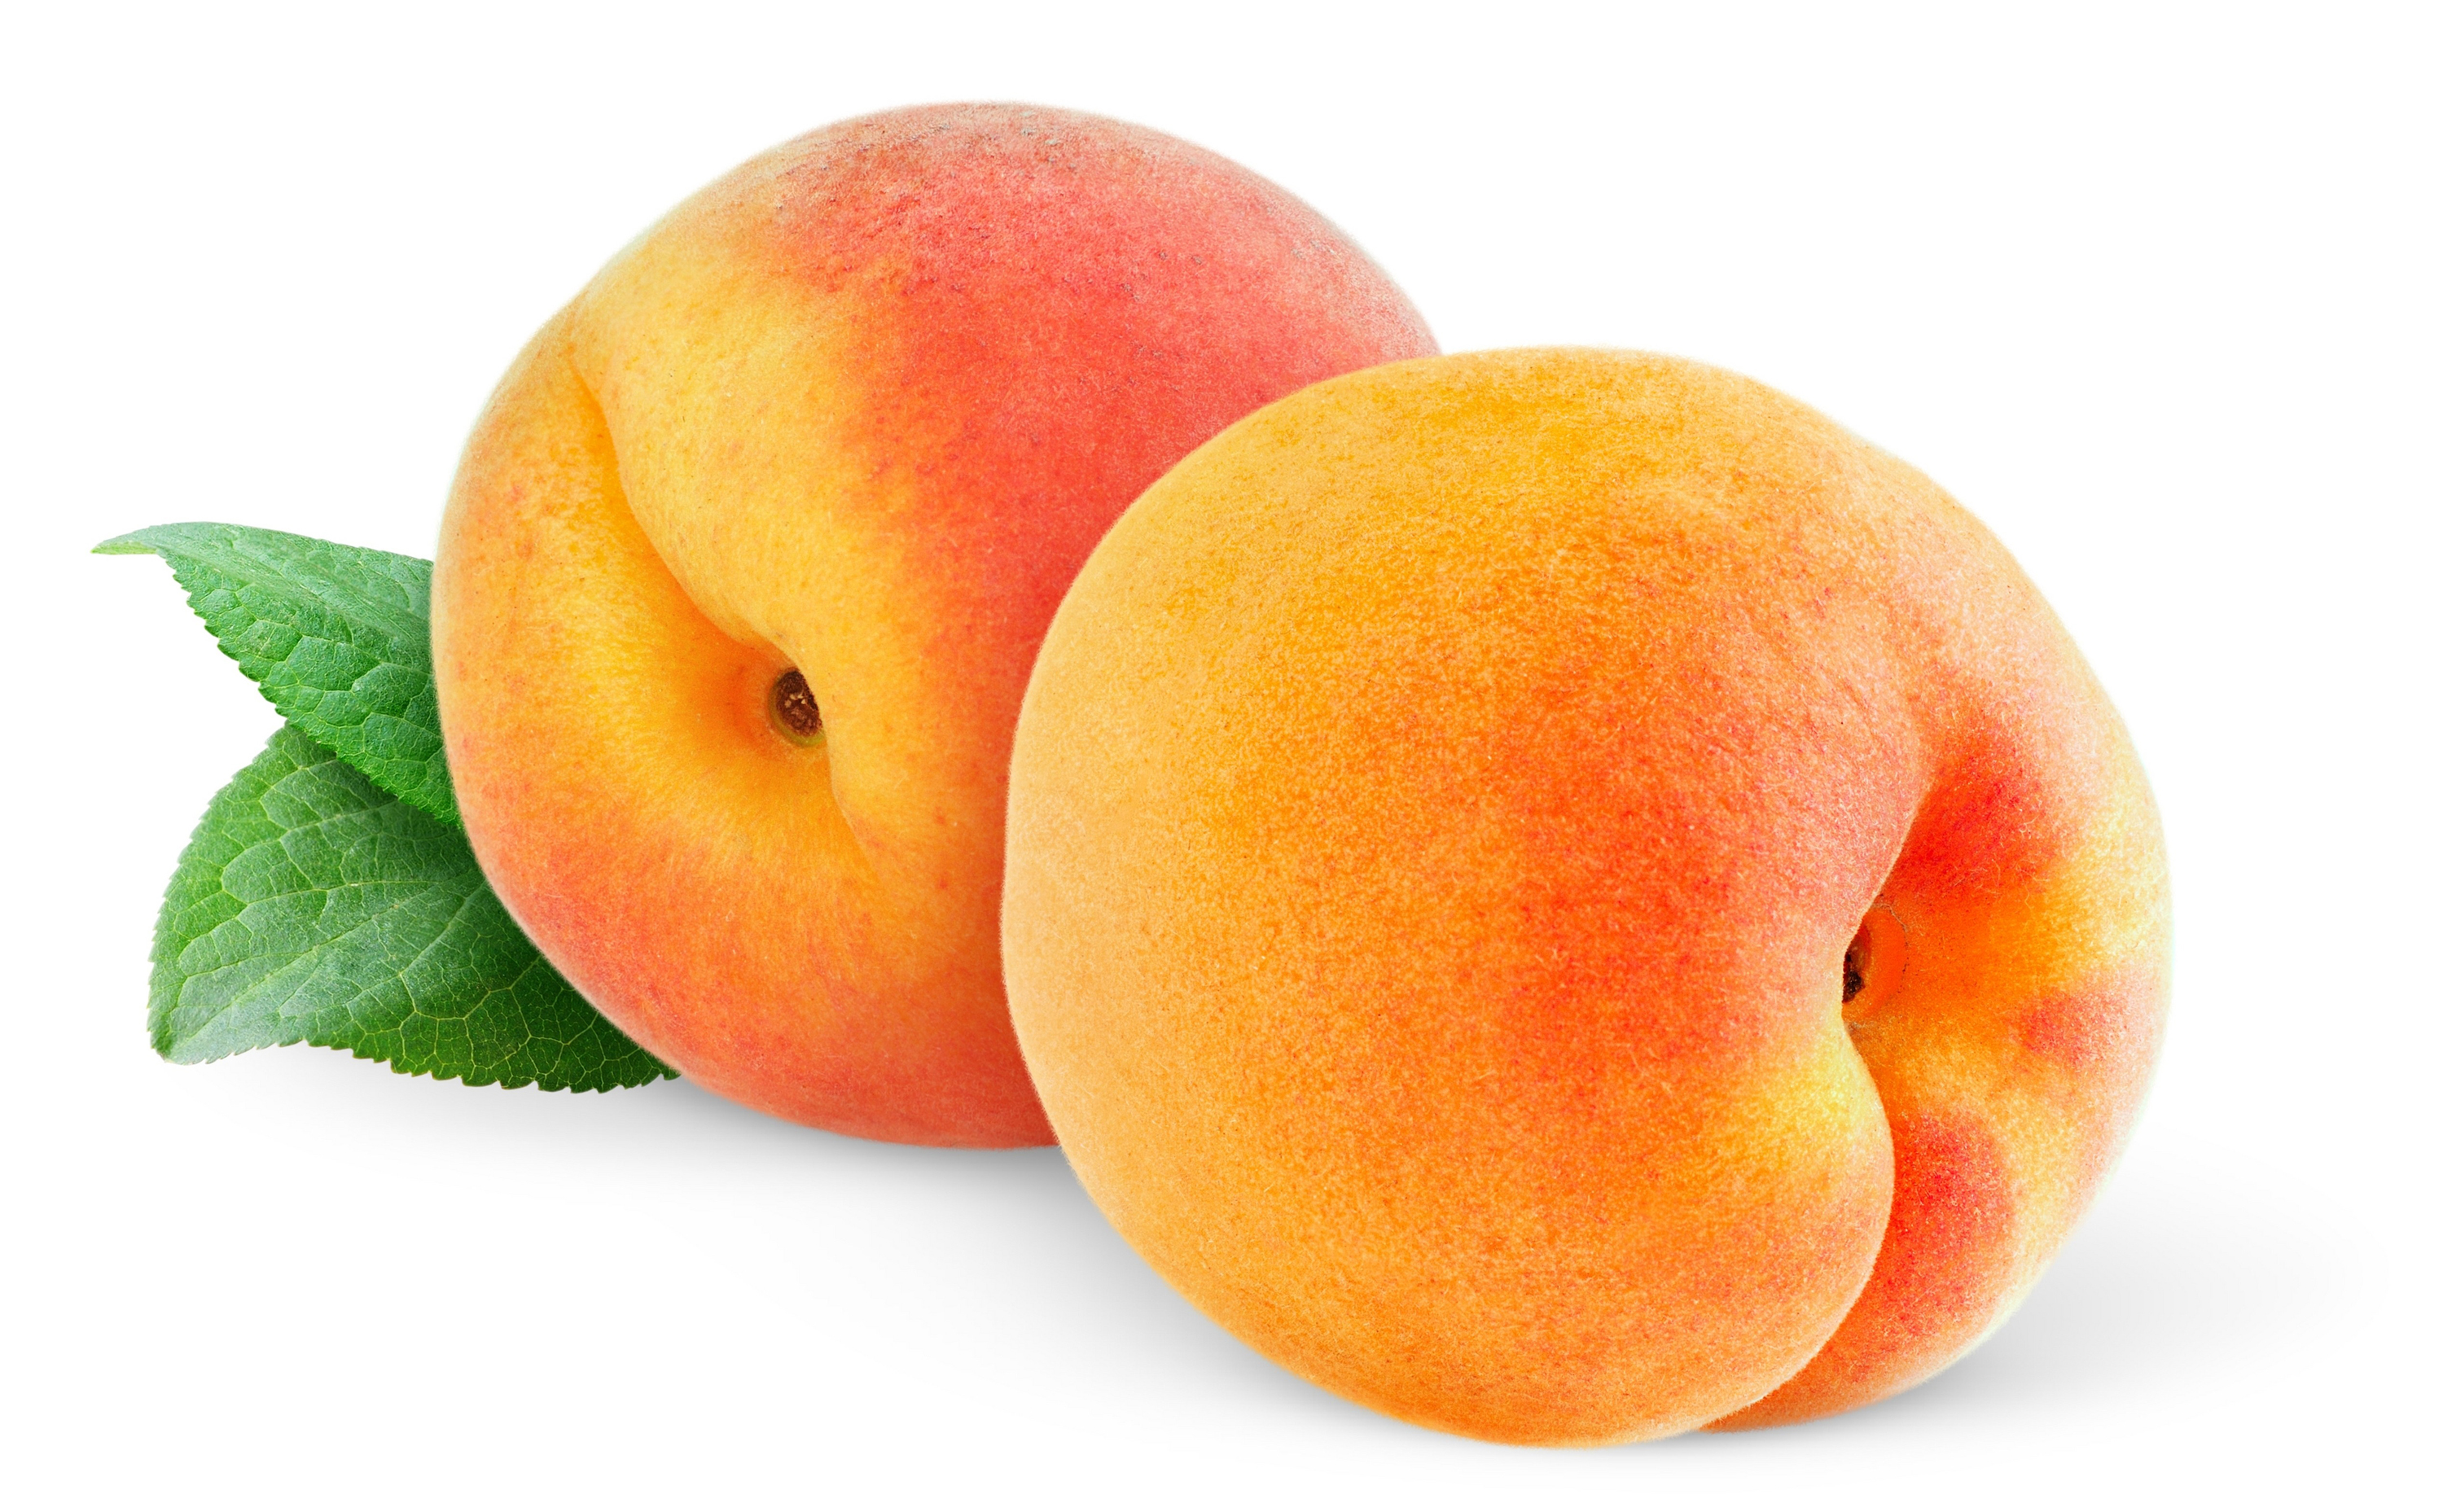
\includegraphics[width=0.8\textwidth]{peachzdfgad.jpg}
  \caption{Delicious peaches although the really new stuff in the paper will be about almonds}
  \label{fig:peach}
\end{figure}
%
\pagebreak
\beginsupplement
\section*{Aknowledgements}
Support for DV provided by the McDonald Endowment for UC Davis Plant Sciences Graduate Student Research Assistantships and the Almond Board of California (ABC; grant HORT16-Aradhya/Ledbetter). Resequencing funded by the ABC (grant HORT16-Aradhya/Ledbetter) and a Henry A. Jastro Research Fellowship. Resequencing funded by the Henry A. Jastro Research Fellowship used the Vincent J. Coates Genomics Sequencing Laboratory at UC Berkeley, supported by NIH S10 Instrumentation Grants S10RR029668 and S10RR027303.
\section*{Supplementary Data}
%somehow change table number also maker table width match full width of text
\begin{center}
\begin{longtable}{lllll}
\caption[P. dulcis, P. persica and related species used in analysis.]{P. dulcis, P. persica and related species used in analysis.} \label{my-label} \\
\hline \hline \multicolumn{1}{l}{\textbf{Sample ID}} &
\multicolumn{1}{l}{\textbf{Accession and/or Cultivar}} &
\multicolumn{1}{l}{\textbf{Origin}} &
\multicolumn{1}{l}{\textbf{Source}}  &
\multicolumn{1}{c}{\textbf{Reference}} \\ \hline 
\endfirsthead

\multicolumn{5}{r}{{\bfseries \tablename\ \thetable{} -- continued from previous page}} \\
\hline \multicolumn{1}{l}{\textbf{Sample ID}} &
\multicolumn{1}{l}{\textbf{Accession and/or Cultivar}} &
\multicolumn{1}{l}{\textbf{Origin}} &
\multicolumn{1}{l}{\textbf{Source}} &
\multicolumn{1}{c}{\textbf{Reference}} \\ \hline 
\endhead

\hline \multicolumn{5}{r}{{Continued on next page}} \\ \hline
\endfoot

\hline \hline
\endlastfoot

                 \multicolumn{5}{l}{\emph{P. dulcis}}  \\
%		 PD01 &DPRU 2578.2 & &NCGR &this study\\
		%Almond Board resequencing (BGI)
		% Not included because it appears to be possible F1 of peach x almond (or reverse)
                 PD02 &‘Tardy Nonpareil’ &USA &UCD &1\\
		%Almond Board resequencing (BGI)
                 PD03 &DPRU 1791.3, BE-1609 &Turkey &NCGR &1\\
		%Jastro resequencing (performed at UC Berkeley)
                 PD04 &DPRU 2374.12 &Iran &NCGR &1\\
		%Jastro resequencing (performed at UC Berkeley)
                 PD05 &DPRU 1456.4, Badam &Pakistan &NCGR &1\\
		%Jastro resequencing (performed at UC Berkeley)
                 PD06 &DPRU 2301, Tuono &Italy &NCGR &1\\
		%Jastro resequencing (performed at UC Berkeley)
                 PD07 &DPRU 1462.2 &Pakistan &NCGR &1\\
		%Jastro resequencing (performed at UC Berkeley)
                 PD08 &DPRU 1207.2 &Uzbekistan &NCGR &1\\
		%Jastro resequencing (performed at UC Berkeley)
                 PD09 &DPRU 2331.9 &China &NCGR &1\\
		%Jastro resequencing (performed at UC Berkeley)
                 PD10 &DPRU 0210, Languedoc &France &NCGR &1\\ %Jastro resequencing (performed at UC Berkeley)
                 PD11 &S3067 &Spain &SRR765861 &2\\
		% resequenced at WSU by Amit Dhingra
                 PD12 &D05-187 &Spain &SRR765850 &2\\
		% resequenced at WSU by Amit Dhingra
                 PD13 &Lauranne &Spain &SRR765838 &2\\
		% resequenced at WSU by Amit Dhingra
                 PD14 &Ramillete &Spain &SRR765679 &2\\
		% resequenced at WSU by Amit Dhingra
                 PD15 &Nonpareil & USA&RosBREED &5\\
                 \\
                 \multicolumn{5}{l}{\emph{P. persica}}  \\ % format italics
                 %PP01 &Lovell &USA &SRR502985 &3\\
                 % resequenced doubled haploid
                 PP02 &Yumyeong &Korea &SRR502994 &3\\
                 PP03 &Shenzhou Mitao&N China &
		\multirow{2}{1cm}{SRR502993, SRR502992} &3\\
                 %honey peach
                 \\
                 PP04 &Sahua Hong Pantao &S China &
		\multirow{2}{1cm}{SRR502991, SRR502990} &3\\
                 %flat peach
                 \\
                 PP05 &Quetta &Pakistan &
		\multirow{2}{1cm}{SRR502989, SRR502987} &3\\
                 \\
                 PP06 &Oro A &Brazil &SRR502986 &3\\
		%
                 PP07 &IF7310828 &Italy &
		\multirow{2}{1cm}{SRR503001, SRR503000} &3\\
                 \\
                 PP08 &GF305 &France &SRR502983 &3\\
                 %
		 PP09 &F$_{1}$ Contender $\times$ Ambra &Italy &SRR502997 &3\\
                 % peach x nectarine both P. persica
                 PP10 &Earligold &USA &
		\multirow{2}{1cm}{SRR502996, SRR502995} &3\\
                %  
		\\
                 PP11 &Bolero &Italy &SRR501836 &3\\
		 %
                 %PP12 &F8,1-42 &USA &SRR068361 &4\\
                 % Nonpareil almond in pedigree
		 % use for introgression investigation
		 PP13 &Georgia Belle &USA &SRR068359 &4\\
		 %
                 PP14 &Dr. Davis &USA &SRR068360 &4\\
		 % 
                 PP15 &Lovell &USA &UCD &1\\
                 % originally a canning variety selected ~1882
		 % currently used as rootstock and/or control for disease screening
                 % FPS, ABC
                 % duplicate cultivar, BGI sequenced at higher depth
                 PP16 &DPRU 1190, Admiral Dewey&USA &RosBREED &5\\
                 %aka PI 673525; introduced 1899
                 PP17 &Babcock &USA &RosBREED &5\\
                 %introduced 1897
                 PP18 &Bolinha &Brazil &RosBREED &5\\
		 % released 1985
		 % parentage: prob OP Aldrighi
		 %(Raseira et al. 1992; http://hortsci.ashspublications.org/content/27/11/1154.full.pdf)
		 %considered resistant to brown rot (Monilinia fructicola); low chill
                 PP19 &DPRU 2142, Carman &USA &RosBREED &5\\
		 %Planted 1889 from OP seed (unknown variety) by J. W. Stubenrauch, Mexia, TX
		 % data entry error listed as Carmen in GRIN; PI book has Carman
		 % http://sun.ars-grin.gov:8080/npgs_public/prodweb.pdf0?in_vol=33&in_suffix=&in_page=052
                 % PI 673586; cultivar original PI 34673 assigned 1912
                 PP20 &Chinese Cling&China &RosBREED &5\\
                 %introduced 1850; founder several cultivars
                 PP21 &Diamante&Brazil &RosBREED &5\\
                 %predominant canning cultivar in Brazil per Okie (year & pub TBD)
                 PP22 &Dixon&USA &RosBREED &5\\
		% Introduced in 1956
		% http://www.google.com/patents/USPP13911
		% early cling peach
                 %PP23 &Dr. Davis& &RosBREED &5\\
                 % duplicate cultivar
                 PP24 &DPRU 0589, Early Crawford &USA &RosBREED &5\\
                 %introduced before 1832
                 PP25 &Elberta&USA &RosBREED &5\\
                 %introduced ~1889; OP sdlg of 'Chinese Cling’
                 PP26 &Florida Prince P138&USA &RosBREED &5\\
                 %low chill cultivar; introduced in 2009
                 %PP27 &Georgia Bell&USA &RosBREED &5\\
                 %(aka ‘Georgia Belle’ and ‘Belle of Georgia’
		% introduced ~1875; OP sdlg of Chinese Cling)
                 %duplicate cultivar
                 PP28 &JH Hale&USA &RosBREED &5\\
                 %male sterile; introduced 1912
                 %PP29 &Lovell &USA &RosBREED &5\\
                 PP30 &Mayflower&USA &RosBREED &5\\
                 %introduced 1909
                 PP31 &Nemaguard &USA &RosBREED &5\\
                 %rootstock; rumored to have P. davidiana in pedigree
                 PP32 &O'Henry &USA &RosBREED &5\\
                 %plant patent 2.964 1/27/1970; OP sdlg Merrill Bonanza; discovered 1960
                 PP33 &Okinawa &Japan &RosBREED &5\\
		% Sharpe 1957
		% http://fshs.org/proceedings-o/1957-vol-70/320-322%20%28SHARPE%29.pdf
		% from 1953 seed lot, different seedlings
		% unsure if only one of these is what is now called 'Okinawa'
		% has nematode resistance
		% used in hybrid combination with Harrow's Blood (F2s) as rootstock
                 PP34 &Oldmixon Free &USA &RosBREED &5\\
                 % introduced 1832
		 % Sir John Oldmixon in the mid 18th century wrote of peach in the Carolinas (Hedrick p50)
                 PP35 &Rio Oso Gem &USA &RosBREED &5\\
                 % introduced 1933
		% developed in Rio Oso, California, Sierra Nevada foothills
		% https://www.slowfoodusa.org/ark-item/rio-oso-gem-peach
                 PP36 &DPRU 2179, Slappey &USA &RosBREED &5\\
                 %aka ‘Slappy’ in GRIN; introduced 1903
                 PP37 &DPRU 0941, St. John Yellow &USA &RosBREED &5\\
                 %introduced 1860s
                 %some variety history at http://gapeaches.org/about-us/father-of-the-ga-peach-industry/
		\\
                 \multicolumn{5}{l}{Other \emph{Prunus} species}  \\
                 %Almond Board resequencing (performed at BGI)
                 PF01 &\emph{P. fenzliana} &? &UCD &1\\
                 %UCD,ABC
                 PG01 &\emph{P. ferganensis} &Fergana Valley &
		\multirow{2}{1cm}{SRR502999, SRR502998} &3\\
                 \\
                 PC01 &\emph{P. cerasifera} DPRU 0579, Myrobalan &USA &NCGR &1\\ \hline
                 %outgroup
                 %NCBI SRA
               %note that the SRR IDs are from NCBI SRA
               %GDR/RosBREED (ftp://ftp.bioinfo.wsu.edu/species/Prunus_persica/RosBREED_Illumina/)

\end{longtable}
\end{center}
$^{1}$ this study\\
$^{2}$ \citealt{koepke2013comparative}?\\
$^{3}$ \citealt{verde2013high}\\
$^{4}$ \citealt{ahmad2011whole}\\
$^{5}$ \url{ftp://ftp.bioinfo.wsu.edu/www.rosbreed.org/resequencing/Prunus_persica/}\\
%\endsupplement
\end{document}
